\documentclass{article}
\usepackage{setspace}
\usepackage{gensymb}
\usepackage{xcolor}
\usepackage{caption}
%\usepackage{subcaption}
%\doublespacing
\singlespacing
\usepackage{float}
\usepackage{graphicx}
%\usepackage{amssymb}
%\usepackage{relsize}
\usepackage[cmex10]{amsmath}
\usepackage{mathtools}
%\usepackage{amsthm}
%\interdisplaylinepenalty=2500
%\savesymbol{iint}
%\usepackage{txfonts}
%\restoresymbol{TXF}{iint}
%\usepackage{wasysym}
\usepackage{amsthm}
\usepackage{mathrsfs}
\usepackage{txfonts}
\usepackage{stfloats}
\usepackage{cite}
\usepackage{cases}
\usepackage{subfig}
%\usepackage{xtab}
\usepackage{longtable}
\usepackage{multirow}
%\usepackage{algorithm}
%\usepackage{algpseudocode}
\usepackage{enumerate}
\usepackage{enumitem}
\usepackage{mathtools}
%\usepackage{eenrc}
%\usepackage[framemethod=tikz]{mdframed}
	\usepackage{listings}
\usepackage{listings}
    \usepackage[latin1]{inputenc}                                 %%
    \usepackage{color}                                            %%
    \usepackage{array}                                            %%
    \usepackage{longtable}                                        %%
    \usepackage{calc}                                             %%
    \usepackage{multirow}                                         %%
    \usepackage{hhline}                                           %%
    \usepackage{ifthen}                                           %%
  %optionally (for landscape tables embedded in another document): %%
    \usepackage{lscape}     
\usepackage{wrapfig}
%\usepackage{ragged2e}
\graphicspath{ {./figs} }
\usepackage{geometry}
\usepackage{multicol}

\SetEnumitemKey{twocol}{
	before=\raggedcolumns\begin{multicols}{2},
	after=\end{multicols}}
\SetEnumitemKey{fourcol}{
	before=\raggedcolumns\begin{multicols}{4},
	after=\end{multicols}}

\geometry{a4paper,total={200mm,225mm},left=25mm,right=30mm}
\begin{document}
\title{CHAPTER 9\\AREAS OF PARLLELOGRAMS AND TRIANGLES}
\maketitle
\section*{EXERCISE 9.1}
Write the correct answer in each of the following:
\begin{enumerate}
\item The median of a triangle divides it into two 
\begin{enumerate}[twocol]
\item triangles of equal area
\item congruent triangles
\item right triangles          
\item isosceles triangles
\end{enumerate}
\item In which of the following figures (Figure 1), you find two polygons on the same base and between the same parallels?
\begin{figure}[!h]
\begin{center}
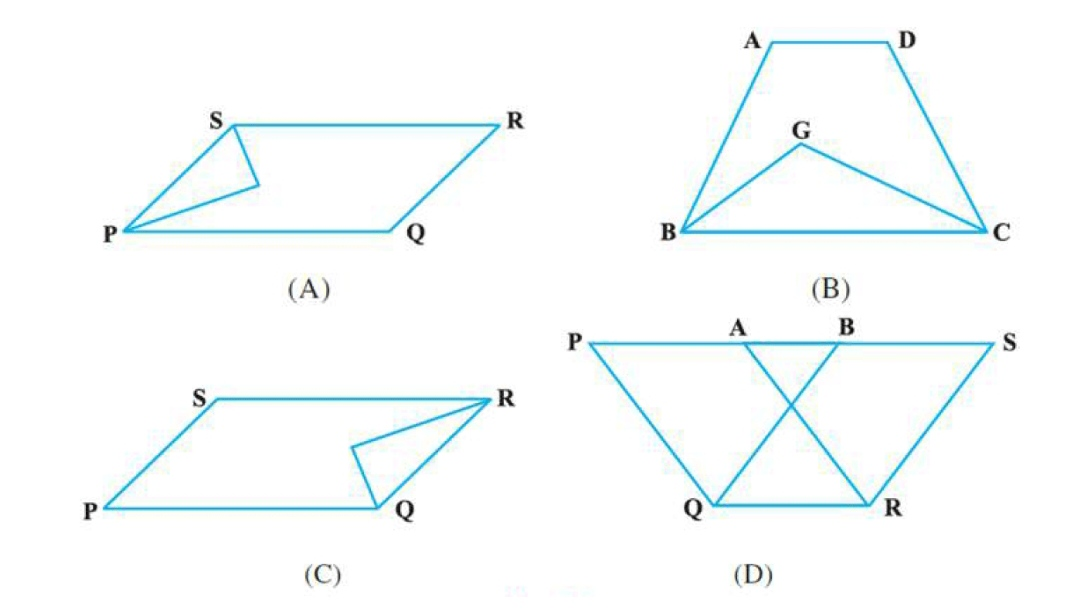
\includegraphics[scale=0.25]{three.jpg}
\end{center}
\caption{}
\label{fig:Fig. 9.3}
\end{figure}
\item The figure obtained by joining the mid-points of the adjacent sides of a rectangle of sides 8cm and 6cm is:
\begin{enumerate}[twocol]
\item a rectangle of area $24 cm^2$ 
\item a square of area $25 cm^2$
\item a trapezium of area $24 cm^2$ 
\item a rhombus of area $24 cm^2$
\end{enumerate}

\item In Figure 2, the area of parallelogram $ABCD$ is:
\begin{figure}[!h]
\begin{center}
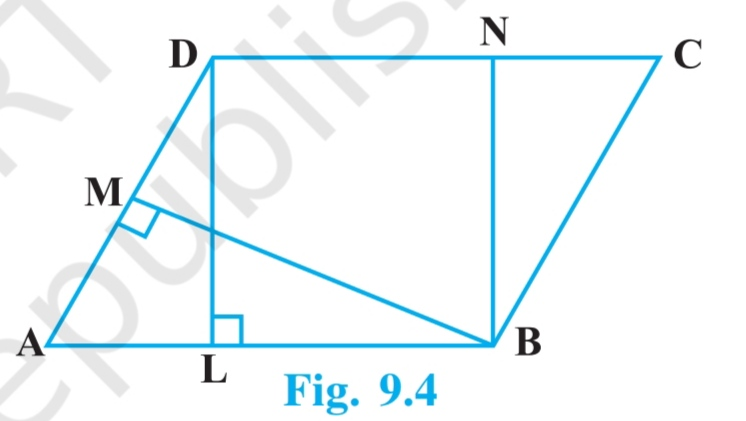
\includegraphics[scale=0.15]{four.jpg}
\caption{}
\label{fig:Fig. 9.4}
\end{center}
\end{figure}
\begin{enumerate}
\item AB x BM
\item BC x BN
\item DC x DL
\item AD x DL
\end{enumerate}
\item In Figure 3, if parallelogram $ABCD$ and rectangle $ABEF$ of equal area, then:
\begin{enumerate}
\item Perimeter of $ABCD$ = Perimeter of $ABEM$
\item Perimeter of $ABCD$ $<$ Perimeter of $ABEM$
\item Perimeter of $ABCD$ $>$ Perimeter of $ABEM$
\item Perimeter of $ABCD$ = $\frac{1}{2}$ (Perimeter of $ABEM$)
\end{enumerate}
\begin{figure}[!h]
\begin{center}
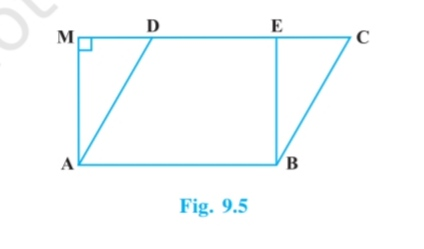
\includegraphics[scale=0.35]{five.jpg}
\end{center}
\caption{}
\label{fig:Fig. 9.5}
\end{figure}
\item The mid-point of the sides of a triangle along with any of the vertices as the fourth point make a parallelogram of area equal to
\begin{enumerate}[twocol]
\item $\frac{1}{2} ar (ABC)$  
\item $\frac{1}{3} ar (ABC)$
\item $\frac{1}{4} ar (ABC)$
\item $ar (ABC)$
\end{enumerate}
\item Two parallelograms are on equal bases and between the same parallels. The ratio of their areas is
\begin{enumerate}[fourcol]
\item $1:2$  \item $1:1$  \item $2:1$  \item $3:1$
\end{enumerate}
\item $ABCD$ is a quadrilateral whose diagonal $AC$ divides it into two parts, equal in area, then $ABCD$
\begin{enumerate}[twocol]
\item is a rectangle       \item is always a rhombus
\item is a parallelogram   \item need not be any of (a), (b) or (c)
\end{enumerate}
\item If a triangle and a parallelogram are on the same base an between same parallels, then the ratio of the area of the triangle to the area of the parallelogram is
\begin{enumerate}[fourcol]
\item $1:3$  \item $1:2$  \item $3:1$  \item $1:4$
\end{enumerate}
\item $ABCD$ is a trapezium with parallel sides $AB = a cm$ and $DC = b cm$ (Figure 4). E and F are the mid-points of the non-parallel sides. The ratio of $ar (ABFE)$ and $ar (EFCD)$ is
\begin{figure}[!h]
\begin{center}
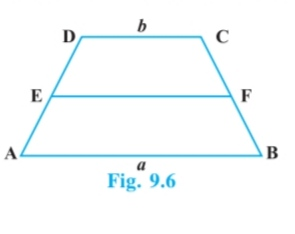
\includegraphics[scale=0.35]{six.jpg}
\end{center}
\caption{}
\label{fig: Fig. 9.6}
\end{figure}
\begin{enumerate}
\item $a:b$ 
\item $(3a+b):(a+3b)$  
\item $(a+3b):(3a+b)$
\item $(2a+b):(3a+b)$
\end{enumerate}
\end{enumerate}

\end{document}
